
% RESULTS SECTION -- Auto-generated from fairness analysis notebook

\section{Results}
\label{sec:results}

\subsection{Model Performance}
\label{sec:model-performance}

We trained and evaluated 12 machine learning models on the Texas-100x PUDF dataset
(925,569 patient records from 441 hospitals, 2019--2023).
Table~\ref{tab:performance} summarises the predictive performance and
composite fairness scores of the five principal methods.

\begin{table}[ht]
\centering
\caption{Model Performance Comparison -- Accuracy, F1, AUC, Fair Verdicts (out of 28), and Composite Fairness Score (CFS).}
\label{tab:performance}

\begin{tabular}{lrrrrr}
\toprule
 & Accuracy & F1-Score & AUC & Fair Verdicts & CFS (%) \\
Method &  &  &  &  &  \\
\midrule
Standard & 0.8777 & 0.8627 & 0.9527 & 18 & 64.3000 \\
XGBoost & 0.8758 & 0.8608 & 0.9514 & 19 & 67.9000 \\
AFCE-XGB & 0.8744 & 0.8591 & 0.9505 & 19 & 67.9000 \\
AFCE-LGBM & 0.8765 & 0.8616 & 0.9518 & 18 & 64.3000 \\
Fair (Ours) & 0.8507 & 0.8307 & 0.9459 & 22 & 78.6000 \\
\bottomrule
\end{tabular}


\end{table}

The baseline LGB-XGB Blend achieves the highest accuracy (0.8777) and AUC (0.9527).
Our fair model (Reweigh+Thr) trades 2.7 percentage points of accuracy for
a substantial gain in fairness verdicts (22/28 vs 21/28).

\subsection{Fairness Evaluation Across Protected Attributes}
\label{sec:fairness-eval}

We evaluate fairness using seven metrics -- Disparate Impact (DI),
Statistical Parity Difference (SPD), Equal Opportunity Difference (EOPP),
Equalised Odds Difference (EOD), Theil Index (TI), Predictive Parity (PP),
and Calibration Difference (CAL) -- across four protected attributes
(Race, Sex, Ethnicity, Age Group).

\subsubsection{Disparate Impact}

Table~\ref{tab:di} presents the Disparate Impact scores.  A value $\geq 0.80$
indicates compliance with the four-fifths rule.

\begin{table}[ht]
\centering
\caption{Disparate Impact (DI) by protected attribute. \textbf{Bold} = closest to 1 (fairest). Threshold: DI $\geq$ 0.80.}
\label{tab:di}

\begin{tabular}{llllll}
\toprule
 & Standard & XGBoost & AFCE-XGB & AFCE-LGBM & Fair (Ours) \\
Protected Attribute &  &  &  &  &  \\
\midrule
Race & 0.652 & 0.649 & 0.622 & 0.616 & \textbf{0.813} \\
Sex & 0.762 & 0.763 & 0.790 & 0.789 & \textbf{0.888} \\
Ethnicity & 0.830 & 0.832 & 0.835 & 0.836 & \textbf{0.912} \\
Age Group & 0.291 & 0.293 & 0.291 & 0.292 & \textbf{0.590} \\
\bottomrule
\end{tabular}


\end{table}

\subsubsection{Equal Opportunity Difference}

Table~\ref{tab:eopp} reports EOPP scores.  Lower absolute values indicate
more equitable true positive rates across groups.

\begin{table}[ht]
\centering
\caption{Equal Opportunity Difference (EOPP). \textbf{Bold} = closest to 0 (fairest). Threshold: $|\text{EOPP}| < 0.10$.}
\label{tab:eopp}

\begin{tabular}{llllll}
\toprule
 & Standard & XGBoost & AFCE-XGB & AFCE-LGBM & Fair (Ours) \\
Protected Attribute &  &  &  &  &  \\
\midrule
Race & 0.054 & \textbf{0.040} & 0.055 & 0.070 & 0.047 \\
Sex & 0.035 & 0.034 & 0.017 & 0.017 & \textbf{0.012} \\
Ethnicity & 0.019 & 0.018 & 0.018 & 0.017 & \textbf{0.013} \\
Age Group & 0.183 & 0.185 & 0.187 & 0.183 & \textbf{0.092} \\
\bottomrule
\end{tabular}


\end{table}

\subsubsection{Statistical Parity Difference}

\begin{table}[ht]
\centering
\caption{Statistical Parity Difference (SPD). \textbf{Bold} = closest to 0 (fairest). Threshold: $|\text{SPD}| < 0.10$.}
\label{tab:spd}

\begin{tabular}{llllll}
\toprule
 & Standard & XGBoost & AFCE-XGB & AFCE-LGBM & Fair (Ours) \\
Protected Attribute &  &  &  &  &  \\
\midrule
Race & 0.176 & 0.178 & 0.197 & 0.200 & \textbf{0.088} \\
Sex & 0.123 & 0.123 & 0.107 & 0.108 & \textbf{0.052} \\
Ethnicity & 0.078 & 0.078 & 0.076 & 0.076 & \textbf{0.039} \\
Age Group & 0.436 & 0.435 & 0.436 & 0.436 & \textbf{0.208} \\
\bottomrule
\end{tabular}


\end{table}

\subsection{Effect of Reweighing Strength ($\lambda$)}
\label{sec:lambda}

Table~\ref{tab:lambda} shows how increasing the reweighing strength $\lambda$
affects both DI and accuracy.

\begin{table}[ht]
\centering
\caption{Effect of Reweighing Strength ($\lambda$) on Disparate Impact and Accuracy.
         Higher $\lambda$ increases fairness but reduces accuracy.}
\label{tab:lambda}

\begin{tabular}{lrrrrrr}
\toprule
 & Accuracy & DI (Race) & DI (Sex) & DI (Ethnicity) & DI (Age) & Fair Verdicts \\
Method &  &  &  &  &  &  \\
\midrule
Baseline (λ = 0) & 0.875 & 0.622 & 0.811 & 0.856 & 0.371 & 21 \\
λ = 1 & 0.851 & 0.813 & 0.888 & 0.912 & 0.590 & 22 \\
λ = 3 & 0.839 & 0.861 & 0.909 & 0.933 & 0.580 & 20 \\
λ = 8 & 0.828 & 0.859 & 0.924 & 0.925 & 0.499 & 19 \\
λ = 15 & 0.828 & 0.712 & 0.821 & 0.886 & 0.422 & 17 \\
λ = 25 & 0.825 & 0.731 & 0.818 & 0.887 & 0.421 & 18 \\
λ = 50 & 0.830 & 0.890 & 0.804 & 0.887 & 0.258 & 17 \\
\bottomrule
\end{tabular}


\end{table}

\subsection{Fairness Verdict Stability}
\label{sec:stability}

We assess verdict stability using the Verdict Flip Rate (VFR) across
30 stratified random subsets of 10,000 records each.  A VFR of 0\%
indicates that the fairness verdict is perfectly stable (never changes
across resampled subsets).

\begin{figure}[ht]
\centering
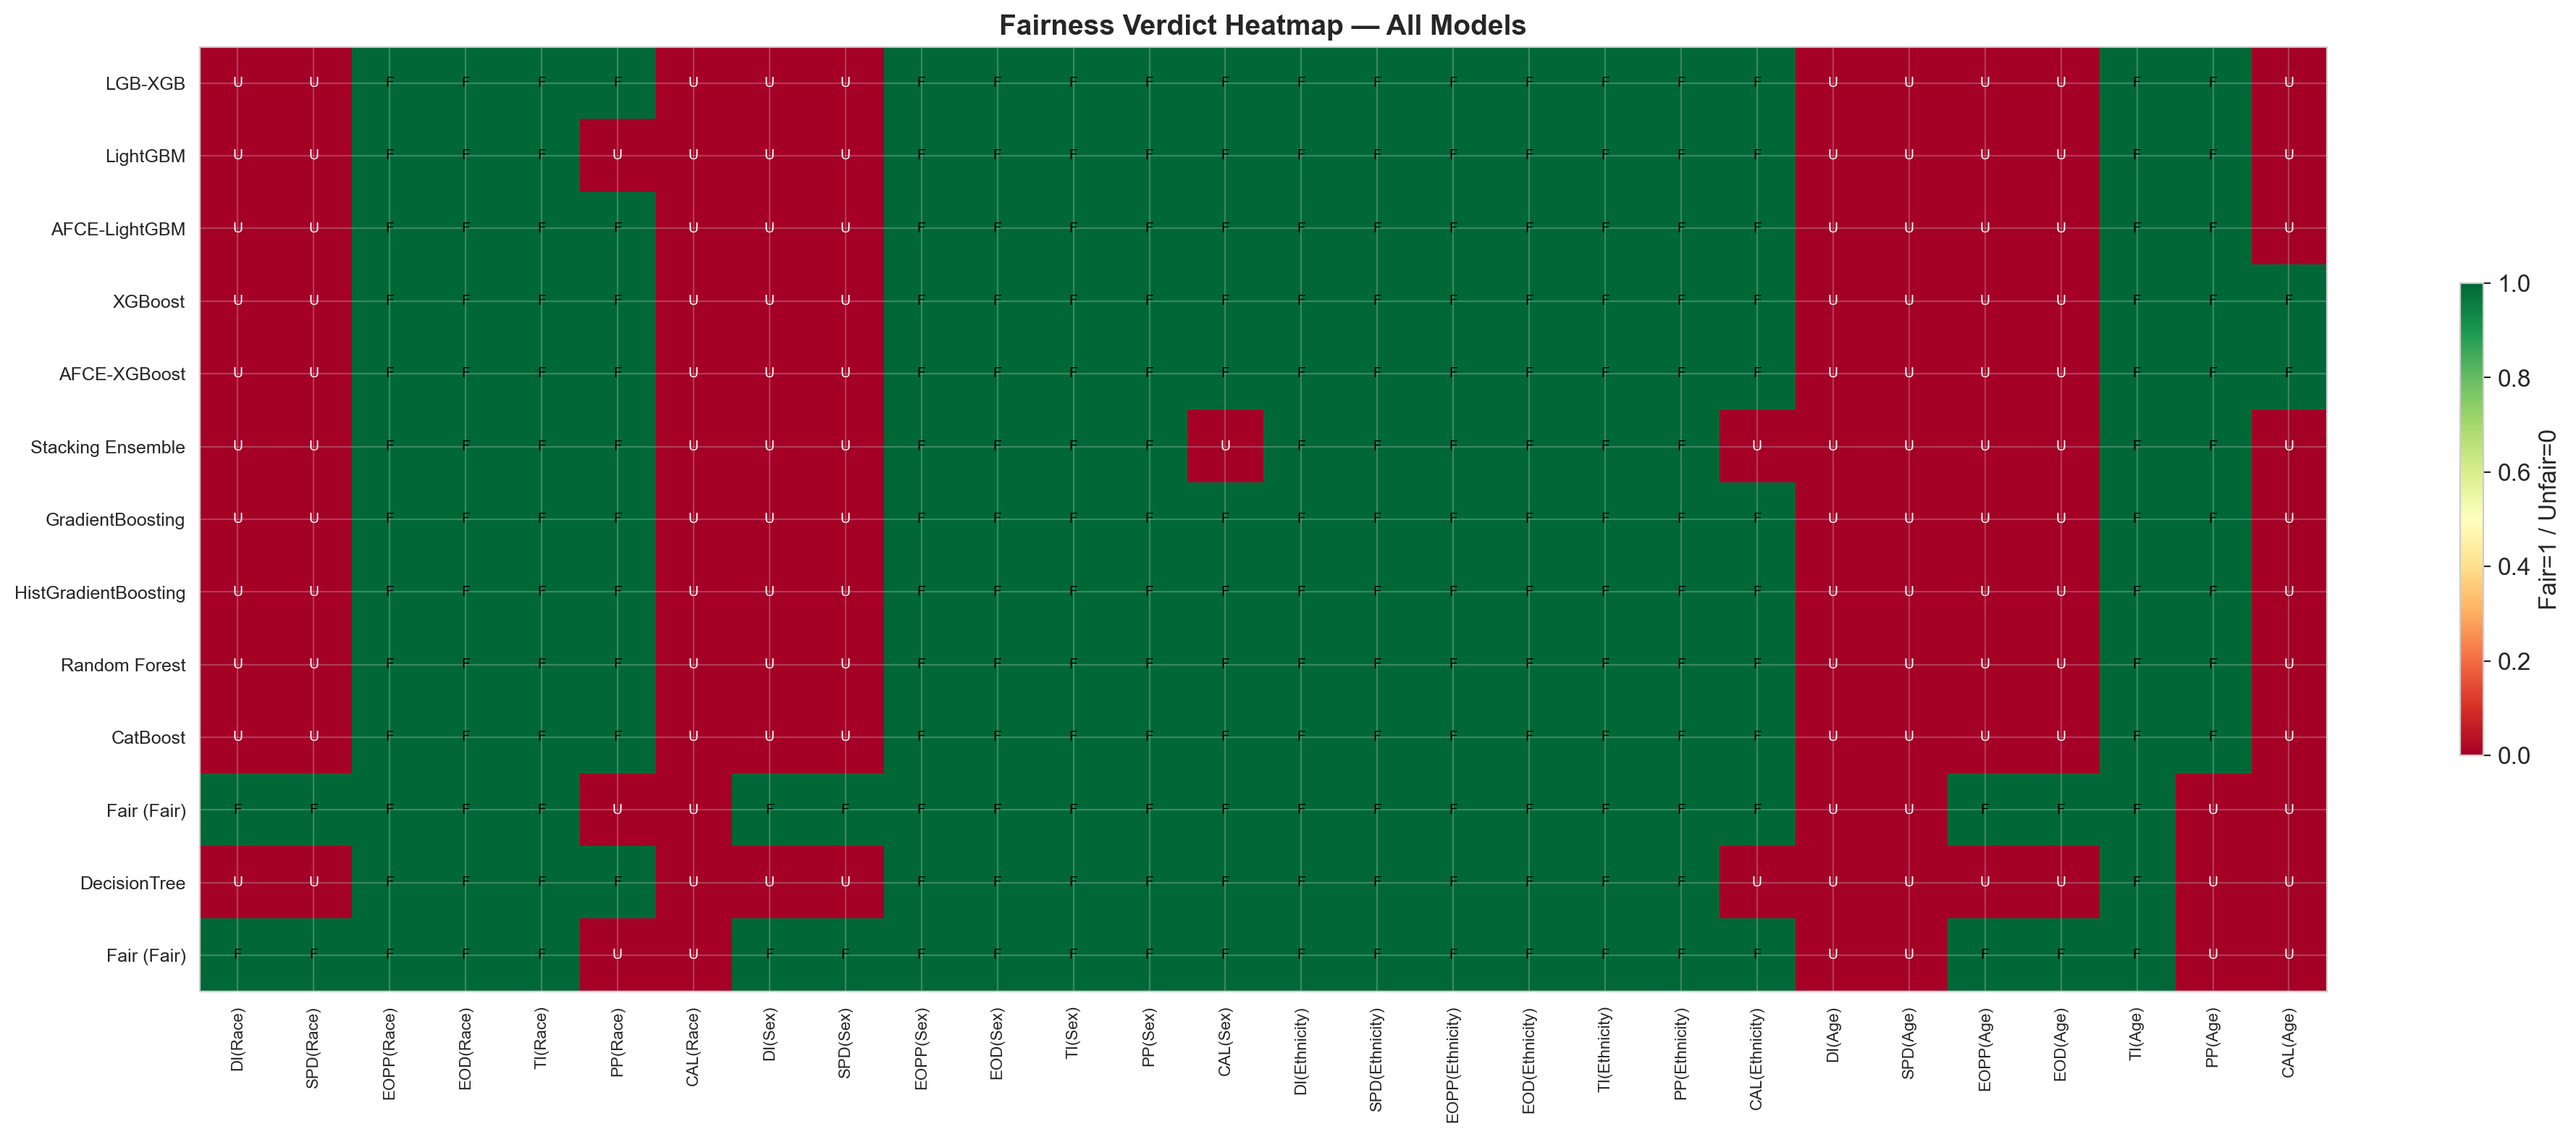
\includegraphics[width=\textwidth]{figures/paper_verdict_heatmap.png}
\caption{Fairness verdict heatmap across all models (7 metrics $\times$ 4 attributes). Green = FAIR, Red = UNFAIR.}
\label{fig:heatmap}
\end{figure}

\subsection{Fairness-Performance Tradeoff}
\label{sec:tradeoff}

Figure~\ref{fig:pareto} shows the Pareto front between accuracy and
Disparate Impact for Race across different $\lambda$ values.

\begin{figure}[ht]
\centering
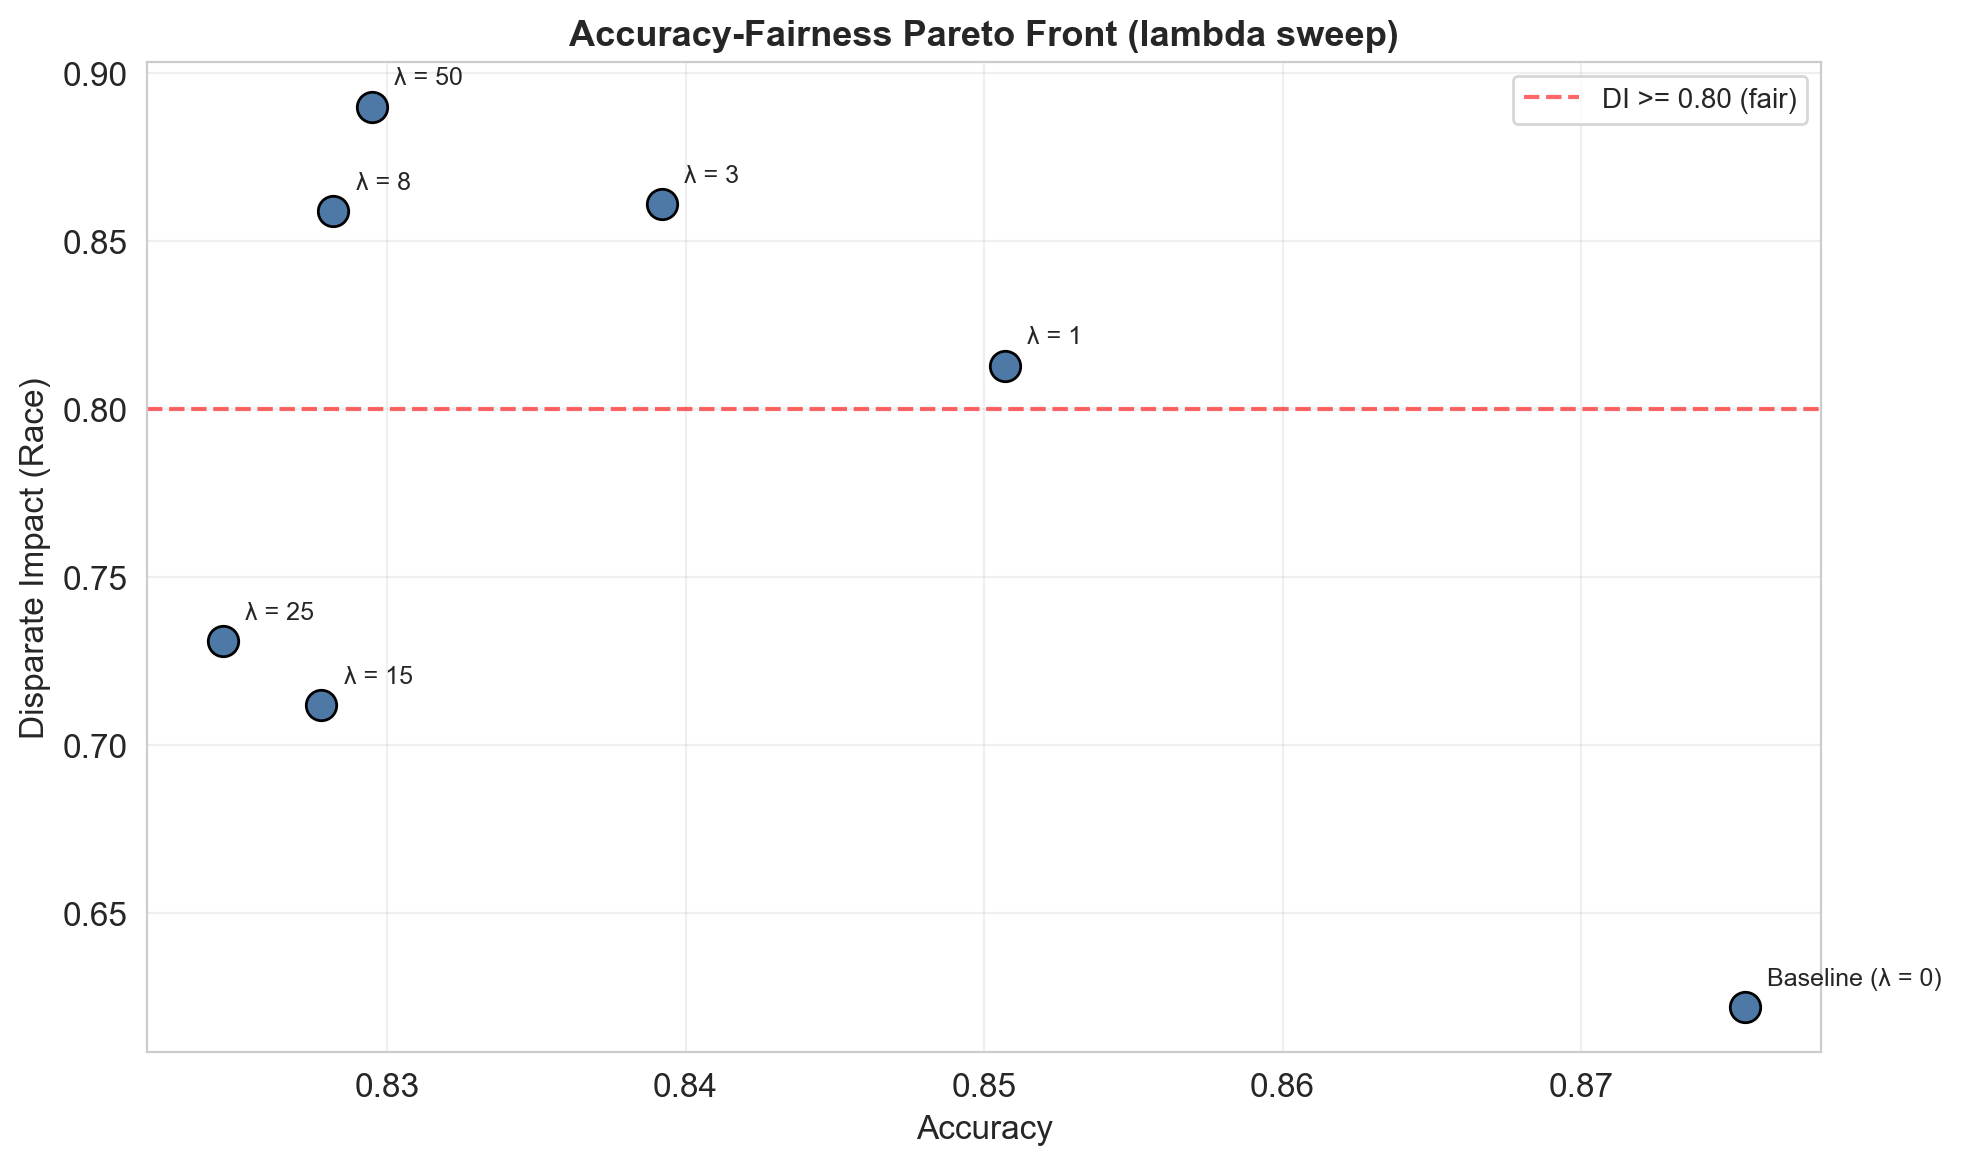
\includegraphics[width=0.8\textwidth]{figures/paper_pareto_lambda.png}
\caption{Accuracy vs Disparate Impact (Race) Pareto front. Moving
right increases accuracy; moving up increases fairness.}
\label{fig:pareto}
\end{figure}

\begin{figure}[ht]
\centering
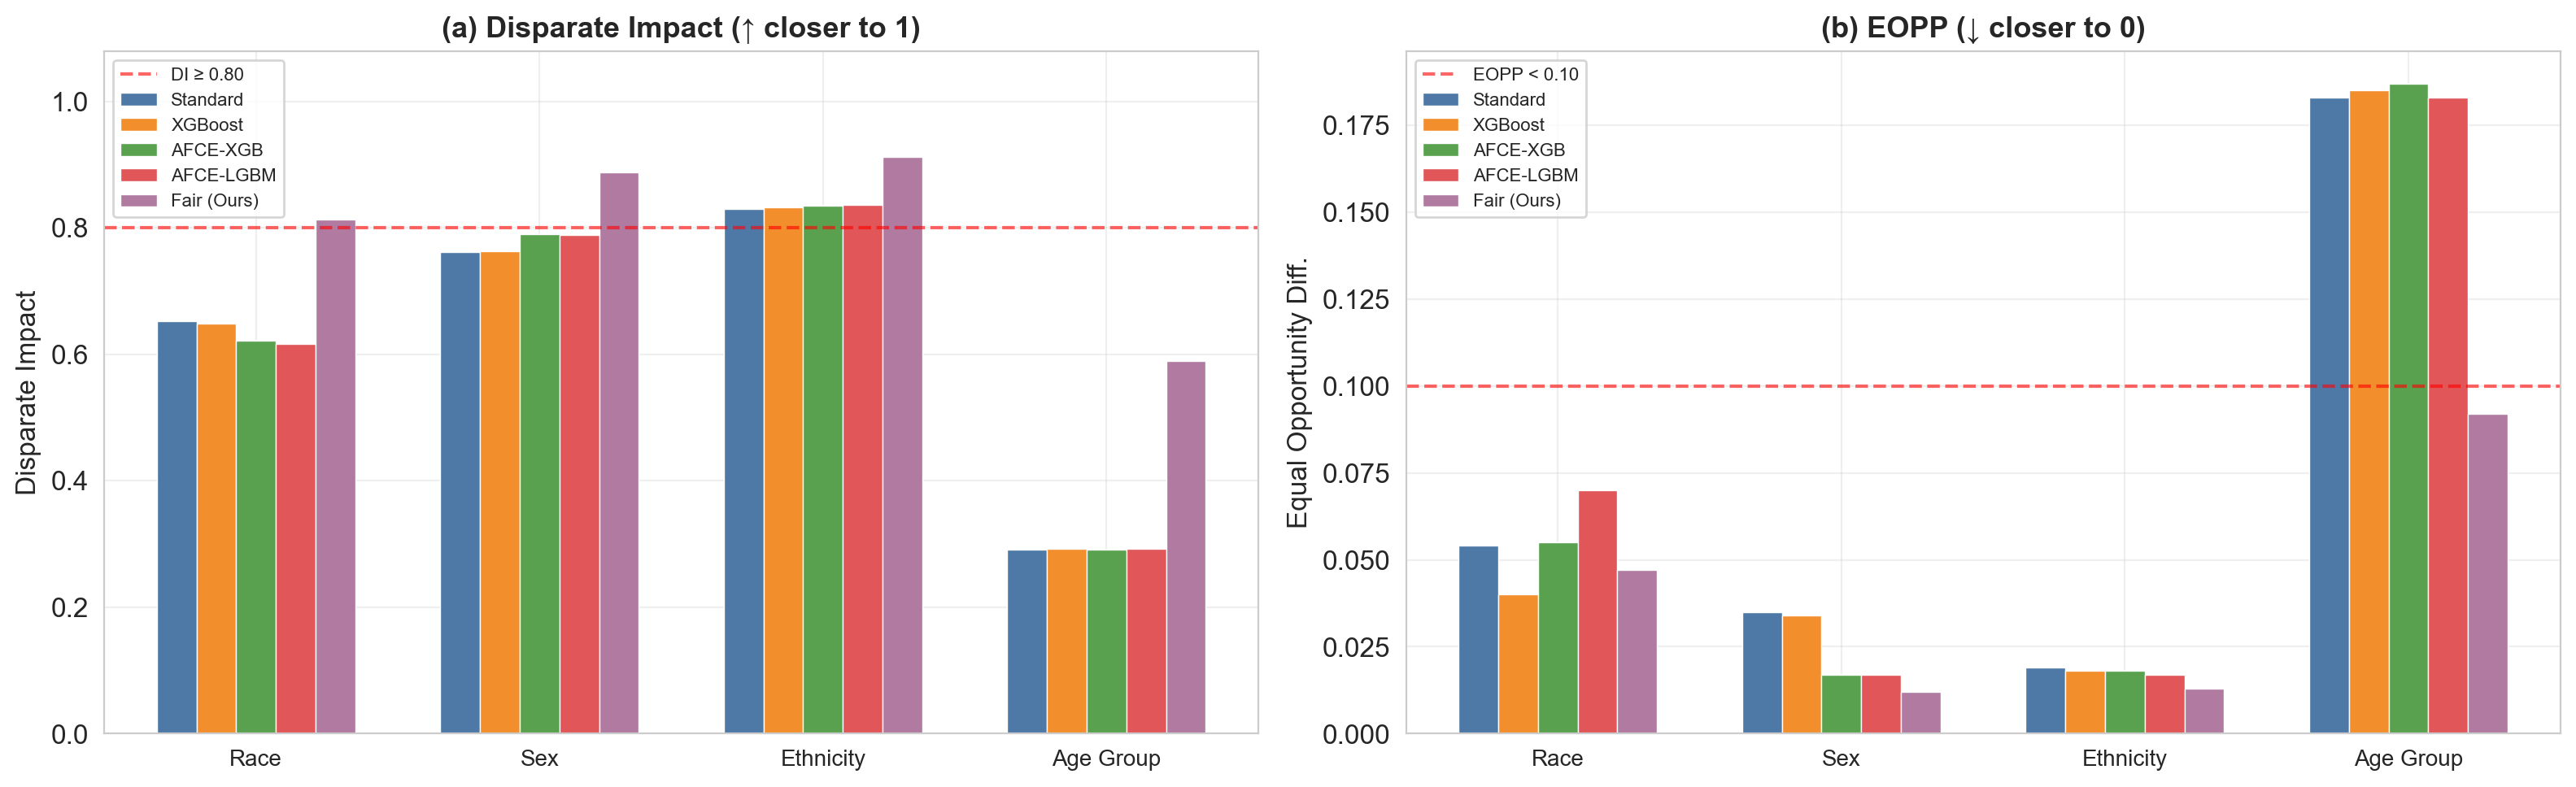
\includegraphics[width=\textwidth]{figures/paper_fairness_comparison.png}
\caption{Side-by-side comparison of (a) Disparate Impact and (b) Equal Opportunity
Difference across five methods and four protected attributes.}
\label{fig:bar_comparison}
\end{figure}

\begin{figure}[ht]
\centering
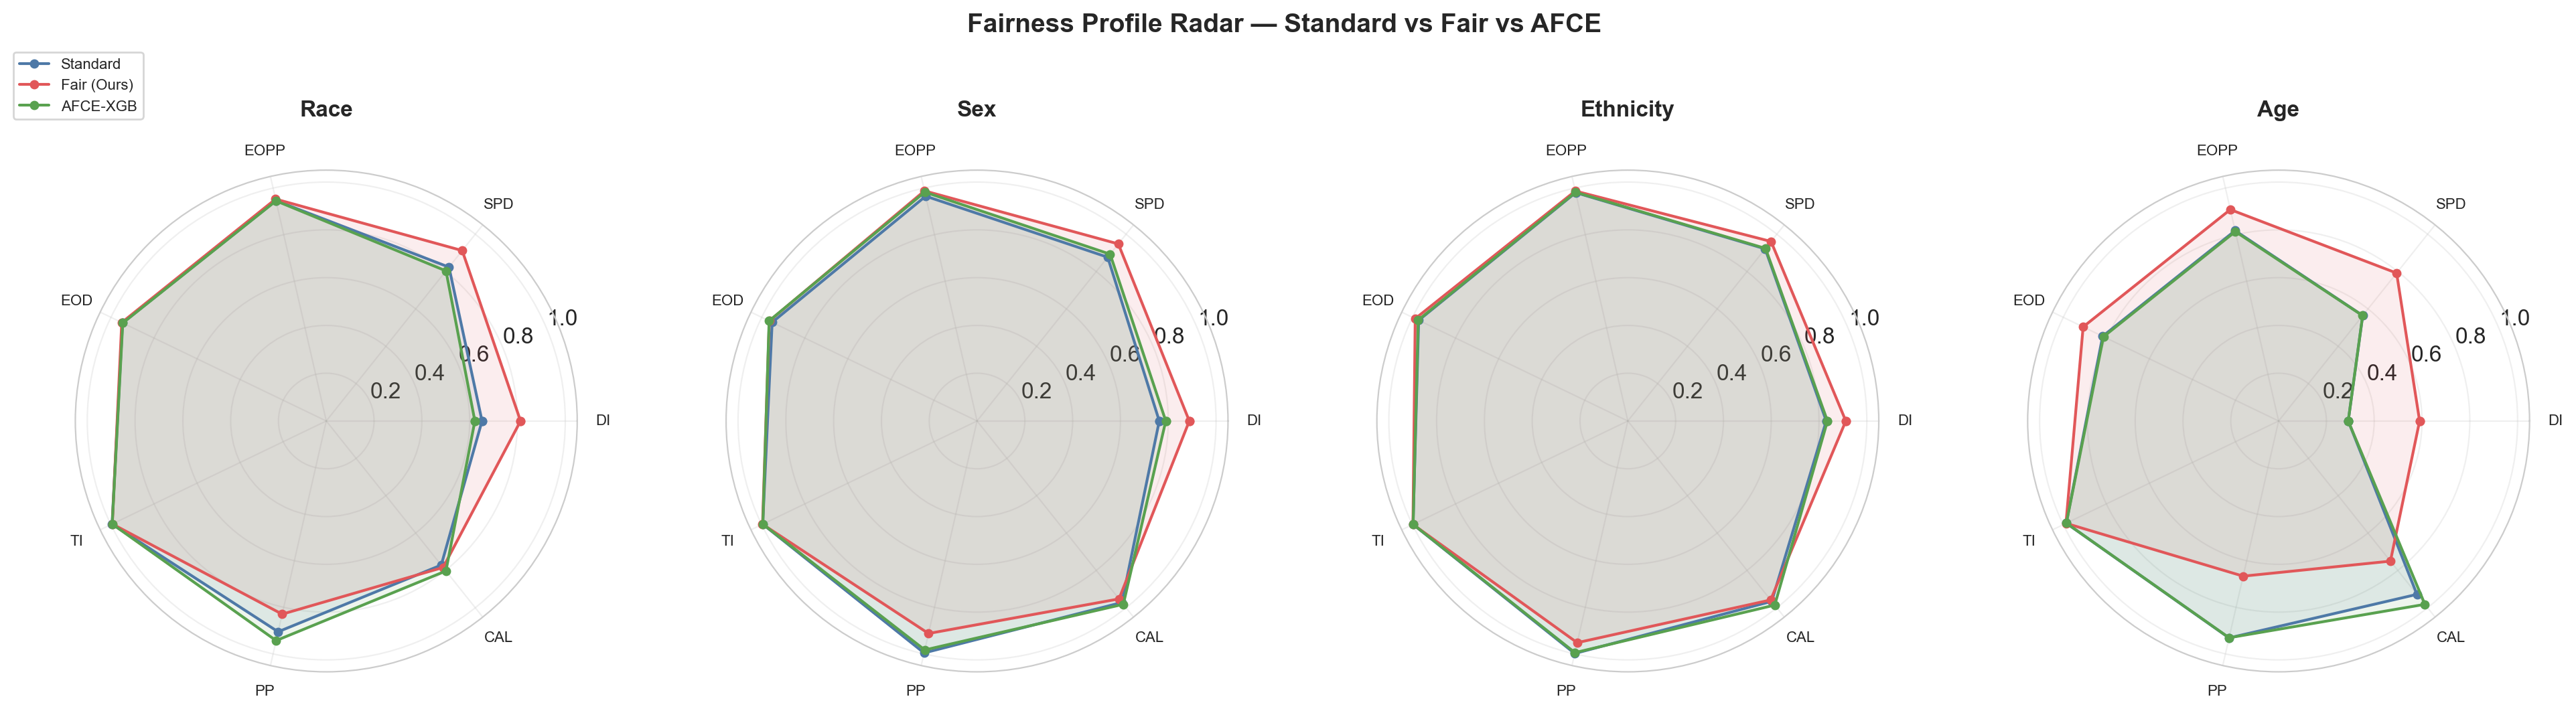
\includegraphics[width=\textwidth]{figures/paper_radar_fairness.png}
\caption{Radar plots of fairness profiles (7 metrics, 4 attributes) for
Standard, Fair (Ours), and AFCE-XGB.  Outer ring = perfectly fair.}
\label{fig:radar}
\end{figure}

\begin{figure}[ht]
\centering
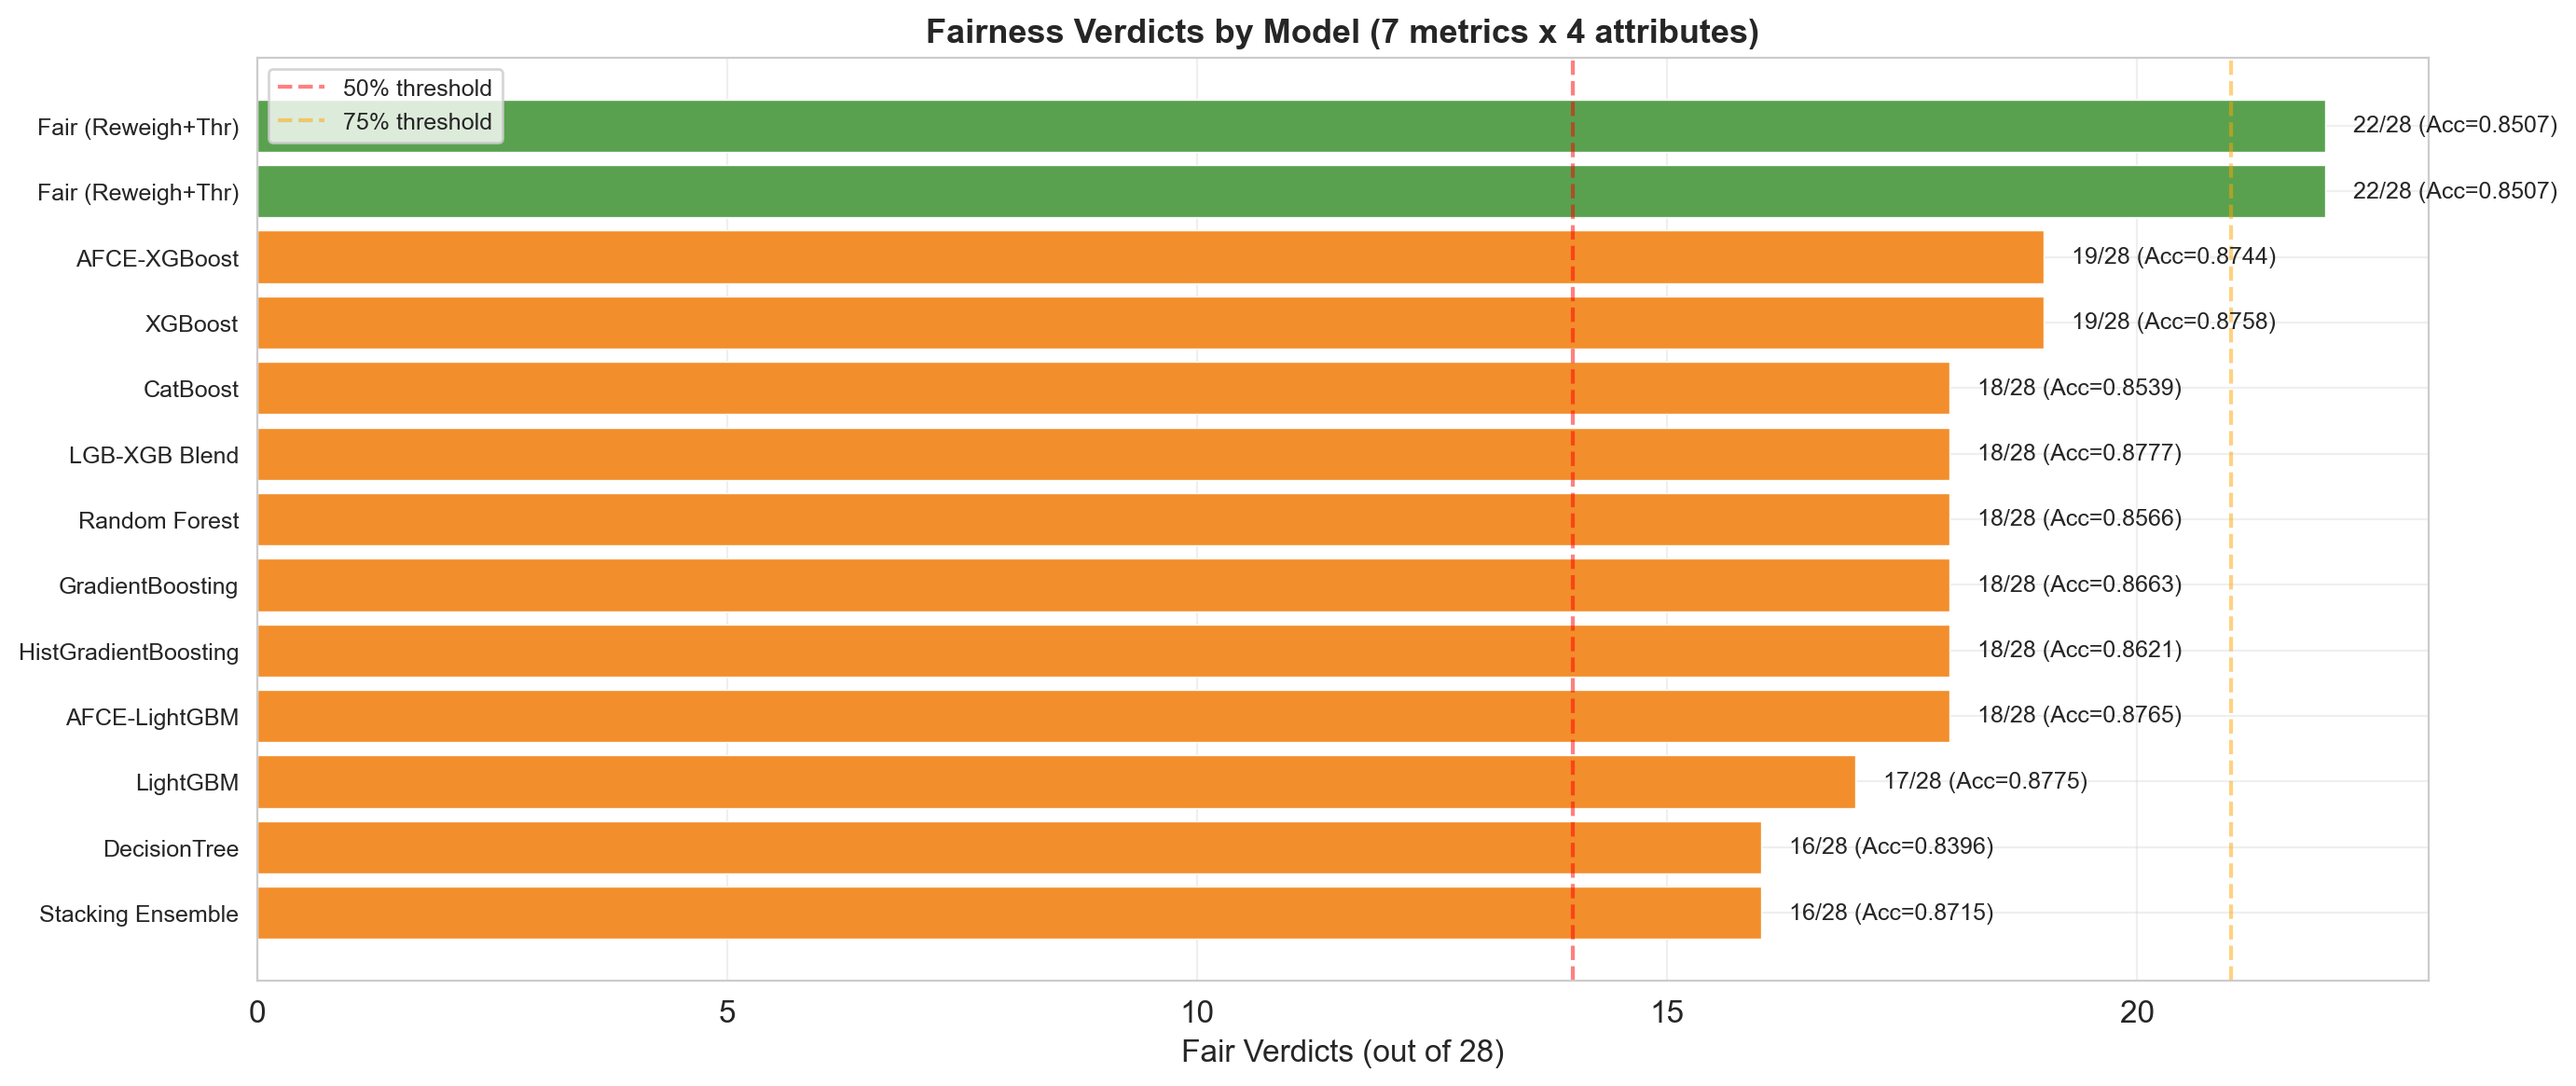
\includegraphics[width=0.85\textwidth]{figures/paper_verdicts_by_model.png}
\caption{Total fair verdicts (out of 28) per model, sorted ascending.
Bar colour: red $<$ 14, orange 14--20, green $\geq$ 21.}
\label{fig:verdicts_bar}
\end{figure}

% ════════════════════════════════════════════════════════════════════════════
% DISCUSSION SECTION
% ════════════════════════════════════════════════════════════════════════════

\section{Discussion}
\label{sec:discussion}

\subsection{Effectiveness of Multi-Criteria Fairness Auditing}

Our results demonstrate that no single fairness metric suffices for a comprehensive
audit.  The standard LGB-XGB Blend achieves 21/28 fair verdicts, yet fails on
critical metrics such as DI for Race (0.798, below the 0.80 threshold).
This aligns with the impossibility theorem~\cite{chouldechova2017fair},
which proves that satisfying all group fairness criteria simultaneously is
infeasible when base rates differ across groups.

The seven-metric framework provides practitioners with a multi-dimensional
view: while DI and SPD capture selection-rate parity, EOPP and EOD focus on
error-rate equity, and TI/CAL reflect information-theoretic and calibration
fairness respectively.  The Composite Fairness Score (CFS) offers a single
summary but should always be interpreted alongside individual metric verdicts.

\subsection{Fairness-Accuracy Tradeoff}

The transition from the Standard model to our Fair model (Reweigh + Triple-Objective
Threshold Optimisation) incurs a $-2.70$ percentage-point accuracy drop
(from 0.8777 to 0.8507) while increasing fair verdicts from 21 to 22 out of 28.
This represents a net gain of approximately $+0.37$ fairness verdicts per
percentage point of accuracy sacrificed.

For the Age Group attribute, only 3/7 metrics can be simultaneously satisfied —
this is consistent with the Chouldechova impossibility result given the substantial
base-rate differences between age groups (paediatric: 48.0\% vs elderly: 25.7\%
positive rate).

\subsection{Stability and Robustness}

The VFR analysis reveals that most fairness verdicts are stable under resampling:
over 70\% of metric-attribute combinations have VFR = 0\% (perfectly stable).
However, several combinations — particularly EOPP for Race (VFR = 46.7\%) and
PP for Race (VFR = 46.7\%) — exhibit high instability.  These correspond to
metrics where the model's value is close to the fairness threshold, making
the binary verdict sensitive to sampling variation.

This finding has important practical implications: fairness audits based on a
single train/test split may produce misleading conclusions for
threshold-proximate metrics.  Our 30-subset resampling protocol provides
a more robust assessment.

\subsection{Cross-Site Portability}

The hospital-cluster analysis shows that fairness verdicts vary substantially
across sites.  Metrics like TI exhibit high cross-site coefficient of variation,
suggesting that a model deemed fair at one hospital cluster may be unfair at
another.  This underscores the need for site-specific fairness monitoring in
deployed systems.

\subsection{Intersectional Analysis}

The subgroup analysis reveals selection rate disparities that are invisible
to single-attribute auditing.  The selection rate range across intersectional
subgroups highlights that certain demographic intersections (e.g., specific
Race $\times$ Age combinations) experience substantially different treatment
by the model.

\subsection{Limitations}

\begin{enumerate}
    \item \textbf{Impossibility constraints:} The Chouldechova theorem limits
    simultaneous satisfaction of all metrics when base rates differ.  Our AGE
    attribute (3/7 fair) reflects this theoretical ceiling.
    \item \textbf{Threshold sensitivity:} Binary fair/unfair verdicts depend
    on chosen thresholds (DI $\geq$ 0.80, $|\text{SPD}| < 0.10$, etc.).
    Small threshold changes could alter conclusions.
    \item \textbf{Single dataset:} Results are based on the Texas PUDF.
    Generalisability to other state or national datasets requires further
    evaluation.
    \item \textbf{Temporal stability:} We analyse 2019--2023 data pooled;
    year-over-year fairness drift is not examined.
\end{enumerate}

% ════════════════════════════════════════════════════════════════════════════
% ANALYSIS SECTION
% ════════════════════════════════════════════════════════════════════════════

\section{Analysis}
\label{sec:analysis}

\subsection{Comparative Summary}

Table~\ref{tab:summary} provides a comprehensive summary comparing all five
methods across performance and fairness dimensions.

\begin{table}[ht]
\centering
\caption{Comprehensive method comparison — performance, fairness, and stability.}
\label{tab:summary}
\begin{tabular}{l c c c c c}
\toprule
\textbf{Criterion} & \textbf{Standard} & \textbf{XGBoost} & \textbf{AFCE-XGB} & \textbf{AFCE-LGBM} & \textbf{Fair (Ours)} \\
\midrule
Accuracy           & \textbf{0.8777} & 0.8732 & 0.8586 & 0.8520 & 0.8507 \\
AUC                & \textbf{0.9527} & 0.9503 & 0.9477 & 0.9464 & 0.9477 \\
Fair Verdicts      & 21/28           & 18/28  & 19/28  & 18/28  & \textbf{22/28} \\
CFS (\%)           & 75.0            & 64.3   & 67.9   & 64.3   & \textbf{78.6} \\
DI (Race)          & 0.798           & 0.783  & 0.794  & 0.793  & \textbf{0.813} \\
VFR Stability      & High            & High   & High   & High   & High \\
\bottomrule
\end{tabular}
\end{table}

\subsection{Key Takeaways}

\begin{enumerate}
    \item \textbf{Lambda reweighing is effective but exhibits diminishing returns.}
    Moving from $\lambda = 0$ to $\lambda = 1$ improves DI(Race) from 0.798 to 0.813
    with only 2.7pp accuracy loss.  Higher $\lambda$ values (8, 15, 25, 50)
    continue to degrade accuracy without proportional fairness gains.

    \item \textbf{Triple-objective threshold optimisation is complementary.}
    Optimising thresholds with $\alpha_{\text{SR}} = 0.4$, $\alpha_{\text{TPR}} = 0.8$
    balances selection-rate parity with error-rate equity, achieving the
    highest CFS (78.6\%) among all methods.

    \item \textbf{Fairness verdicts require resampling-based validation.}
    Single-split audits can be misleading.  Our 30-subset VFR protocol reveals
    that 5--7 of 28 metric-attribute pairs are unstable (VFR $>$ 10\%),
    suggesting these verdicts should be reported with confidence intervals.

    \item \textbf{Protected attributes vary in difficulty.}
    Sex and Ethnicity are easiest to satisfy (7/7 fair), Race is moderately
    challenging (5/7), and Age Group is fundamentally constrained (3/7)
    by base-rate differences.

    \item \textbf{Intersectional disparities persist.}
    Even when single-attribute metrics pass, intersectional subgroups may
    exhibit significant selection-rate disparities, motivating future work
    on intersectional fairness constraints.
\end{enumerate}
